\subsection{Decision and control layers}

For this work, two layers of intelligence are provided. One dealing with the revenue maximisation problem, which returns the assignment of clients to the rooms according to the booking characteristics and the commercial description of the rooms involved in the building. The second layer represents a lower level optimal control problem that ensures minimal energy consumption for an imposed maximum revenue and which depends on the topology and adjacency relationships within the rooms, exterior and ground.

With consideration of the sets:

\begin{align*}
& d \in D=\{0, 1, ...n_d\}\\
& r \in R=\{0, 1...n_c, n_c+1 ... n_s ... n_r \}=\bigcup\{R_c,R_s\}\\
& R_d \subseteq R\\
& R_{dn} = R_d \bigcup {\gamma} \\
& d \in D_d \subseteq D\textbackslash d\\
& t \in T_1=\{1...N\}\\
& t \in T_2=\{1...N+1\}\numberthis
\end{align*}

described by booking requests set $D$, $R$ available $n_r$ rooms in building, out of which there are $n_c$ client rooms and $n_s$ service rooms or common areas (corridors and lounges), $R_d$ compatible rooms to request $d$ (in the case of considering the dummy node $\gamma$, one considers $R_{dn}$), the time sets $T_1$ and $T_2$ for revenue and energy consumption optimisation problems respectively and $D_d$ competing requests of request $d$.

The corresponding constants defined for this step of development are:
\begin{align*}
& T_{sp} = 20\\
& \hat{T}_{i,1}\\
& q^S_{i,t} \text{, } T_{e,t}\\
& K_{i,j} \text{ and } c_{i} \forall i,j\mid i,j\in R \text{, } i\sim j \numberthis
\end{align*}

where $T_{sp}$ determines the temperature setpoint to be reached when a room is selected. The initial temperature states of each room are imposed to be $\hat{T}_{i,1}$. The exogenous inputs $q^S_{i,t}$ and $T_{e,t}$ correspond to the solar radiation through the windows of each room differentiated according to its position on the Earth and the external temperatures measured at every sample. Finally, the transmittance and capacitance parameters $K_{i,j}$ and $c_i$ obtained either through initial theoretical estimate or  parameter identification routines.

With this information, the decision variables used for the solution of both optimisation problems are:
\begin{align*}
& x_{d,r}\in\mathbb{B} \text{ }\forall d\in D \text{ and } r\in{Rd}\bigcup \{\gamma\}\\
& z_{i,t}\in\mathbb{B} \text{ }\forall i\in{Rd} \text{ and }t\in T\\
& T_{i,t}\in\mathbb{C} \text{ }\forall i\in{Rd} \text{ and }t\in T\\
& u_{i,t}\in\mathbb{C} \text{ }\forall i\in{Rd} \text{ and }t\in T\numberthis
\end{align*}

The complete optimisation problem with emphasis on its linear multi objective nature is shown in Eq.~\ref{eq:opt_multi}.

 \begin{flalign*}
 &\begin{array}{rlclcl}
 \displaystyle Y^*=\max_{x_{d,r}} & \multicolumn{3}{l}{\sum_{d\in D}\sum_{r\in R_d}Y_{d,r}x_{d,r}} \\
 \textrm{s.t.} & \sum_{r\in R_{dn}}x_{d,r}=1 \text{ }\forall d\in D \\
 & x_{d,r}+x_{k,r}\leq 1 \text{ } \forall d\in D\text{, }\forall k\in D_d\\
 & \text{ and } \forall r\in R_d\cap R_k
 \end{array}\\
  &\begin{array}{rlclcl}
  \displaystyle E^*=\min_{x_{d,r}} & \multicolumn{3}{l}{\sum_{t\in T}\sum_{i\in R}u_{i,t}} \\
  \textrm{s.t.} & \sum_{r\in R_{dn}}x_{d,r}=1 \text{ }\forall d\in D \\
  & x_{d,r}+x_{k,r}\leq 1 \text{ } \forall d\in D\text{, }\forall k\in D_d\\
  & \text{ and } \forall r\in R_d\cap R_k\\
  & z_{i,t} = \sum_{\substack{d\in D\\t_d^{in}\leq t \leq t_d^{out}}} x_{d,r} \text{ } \forall r\in R \text{, }\\
  &\forall t\in{T_1}\\ 
  & \hat{T}_{i,t+1}=\frac{1}{c_i}(\sum_{i\sim j\bigcup e}(\hat{T}_{i,t}-\hat{T}_{j,t})+\\
  & K_{u}u_{i,t}+q^S_{i,t}+\hat{T}_{i,t})\\
  & T_{i,1} = \hat{T}_{i,1}\\
  & u_{i,t}\geq 0\\
  & u_{i,t}\geq z_{i,t}(T_{sp}-T_{i,t})\\
  & z_{j,t} \geq \wedge z_{k,t} \text{ }\forall j\in{R_{s}} \text{ and }k\sim j\\
  & Y_{t}\geq Y^*
  \end{array}\\
  & \numberthis
 \label{eq:opt_multi}
 \end{flalign*}
 
 The aim of this multiobjective problem is that of generating optimal energetically performing assignments once the revenue was maximised. With this a clear differentiation between actual solvers in the market and this scheduling system can be highlighted. For the development of this task, the work is divided into the next steps:
 \begin{enumerate}
 	\item Solution of the revenue maximisation assignment problem (upper bound on revenue).
 	\item Generation of additional revenue-wise optimal solutions 
 	\item Determination of the energy consumption of each of the obtained solutions. (Energy efficiency estimation).
 	\item Solution of the energy consumption minimisation problem (energetical lower bound on maximal revenue solution).
 \end{enumerate}
 
 Notice than the profit is redefined to be depending on the kind of assignments $x_{d,r}$ performed instead of on attempting only to maximize income, which is also something that many easy solvers do. For this, six levels of profit were proposed, each for the compatible assignment of three levels of clients to three levels of rooms and accordingly to Table~\ref{tab:profits}.
 \begin{table}[htbp]
 	\centering
 	\caption{Levels of profits used as a marketing strategy for this work}
 	\begin{tabular}{cr|ccc}
 		\toprule
 		\multicolumn{2}{c|}{\multirow{2}[0]{*}{Request}} & \multicolumn{3}{c}{Room type} \\
 		\multicolumn{2}{c|}{} & Low  & Medium & High \\ 
 		\midrule
 		\multirow{2}[0]{*}{} & Low &   9   &   7    & 2 \\
 		& Medium &   0    &   22    &  17\\
 		& High &0 & 0& 72\\
 		\bottomrule
 	\end{tabular}%
 	\label{tab:profits}%
 \end{table}%
 
 The profit was proposed in representative costs, not related to the real world and chosen with the proposal of a desired probability distribution to allow for approachability into a more real scenario. Notice that this profit definition does not suppress the possibility of assignment of high level rooms to low level requests, for which it is also possible to include an intelligent offer for the clients to ensure their pleasure as much as these profit values are tuned. As an example, one could consider the hotel in Fig.~\ref{fig:smallhotel} with rooms 5 and 6 categorised as a high level rooms and rooms 9 and 10 with the biggest amount of solar irradiation (therefore energetically less demanding, at least in a direct sense).
 
    \begin{figure}[thpb]
    	\centering
    	\framebox{\parbox{3in}{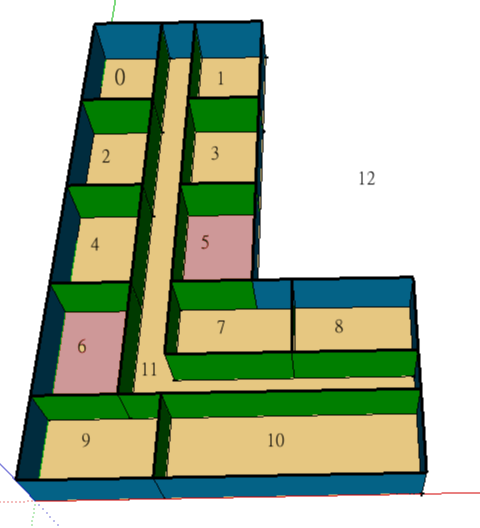
\includegraphics[width=77mm]{img/small_hotel.png}}}
    	%\includegraphics[scale=1.0]{figurefile}
    	\caption{Forward simulation of the system after parameter identification.}
    	\label{fig:smallhotel}
    \end{figure} 
    
After running the framework, one can find, among the several solutions, that by ensuring the optimum revenue value, it is possible to get energetically less demanding solutions preferring to start assigning rooms near rooms 9 and 10 than farther away. Notice that for this case, the fact that one room is occupied implies that the temperature of the central corridor (11) is also set to $T_{sp}$ so that it might become more difficult to give a direct interpretation of the solutions. Nevertheless, the optimisation framework approach corresponds to a software robot capable of deciding for the owner of the building which rooms to assign by protecting the revenue, ensuring least energy consumption and learning the real parameters of the system for further proposals.